%?????????????????????????
% Nombre: capitulo3.tex  
% 
% Texto del capitulo 3
%---------------------------------------------------

\chapter{Clasificaci�n con Redes Neuronales}
\label{nn}

En este cap�tulo veremos el proceso seguido y las distintas vertientes de entrenamiento usadas a lo largo de la realizaci�n de la pr�ctica. Concretamente veremos los resultados en funci�n de la metodolog�a y  topolog�as usadas. 

\section{From Scratch}

\section{Transfer Learning}

Para probar este punto hemos seguido la idea que puede verse en el siguiente c�digo de github \cite{tutorial3}. En el se usa la red Inception\_BN, que es el estado del arte en clasificaci�n de la bater�a de im�genes \textit{\textbf{imagenet}}, para clasificar las im�genes de nuestro problema.  Este problema, tiene cientos de  clases correspondientes a diferentes objetos u animales y clasifica una foto en funci�n a estas, dado que nosotros tenemos entre manos objetos del mundo real y no son muy t�cnicos esta soluci�n nos pareci� al menos digna de tener en cuenta. 

Los resultados obtenidos por este modelo de procesado son aceptables en im�genes sencillas donde las clasifican claramente como armas de fuego, pistolas, rifles de asalto o smartphones pero hay otros casos mas complejos y especiales del dominio del problema cuya clasificaci�n falla, debido a esto esta opci�n queda descartada ya que para obtener buenos resultados en la competici�n no podemos quedarnos con clasificar bien la mayor�a de im�genes sencillas sino que deber�amos aprender tambi�n las complejas.

 A continuaci�n y a modo de ejemplo podemos ver algunas im�genes que se han clasificado y la salida dada por el modelo:

\begin{figure}[H]
	\centering
		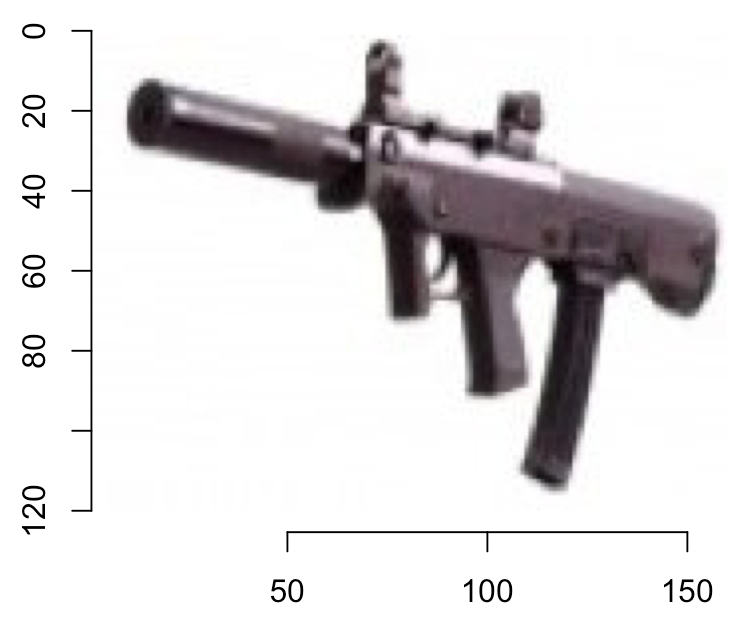
\includegraphics[scale=0.4]{./Capitulo3/imagenes/1.png}
		\caption{Imagen de pistola, clasificada como Assault Rifle.}
	\label{1}
\end{figure} 


\begin{figure}[H]
	\centering
		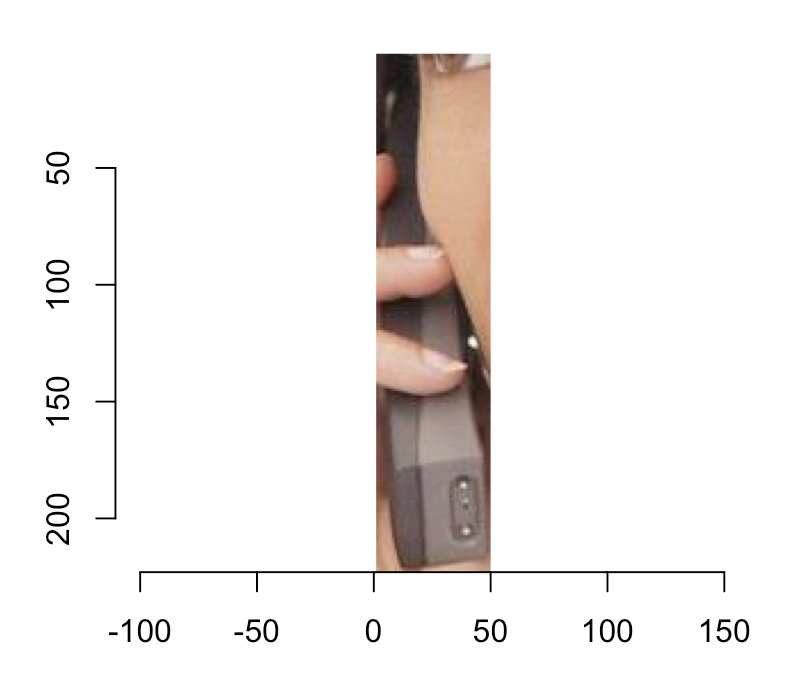
\includegraphics[scale=0.4]{./Capitulo3/imagenes/2.png}
		\caption{Imagen de tel�fono, clasificada como Window Screen.}
	\label{2}
\end{figure} 


\begin{figure}[H]
	\centering
		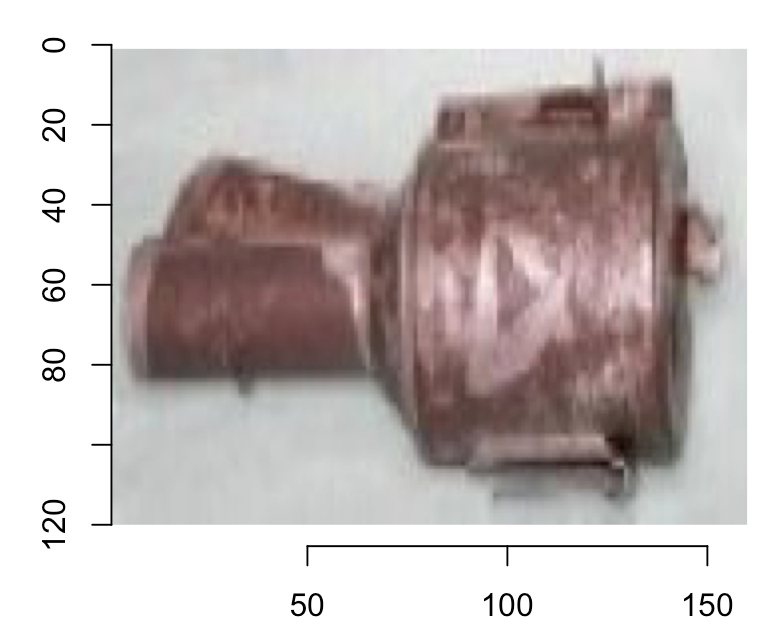
\includegraphics[scale=0.4]{./Capitulo3/imagenes/3.png}
		\caption{Imagen de arma, clasificada como Barril.}
	\label{3}
\end{figure} 


\section{Fine Tunning}

\pagebreak
\clearpage
%---------------------------------------------------